\documentclass[journal]{IEEEtran}
\usepackage[a5paper, margin=10mm]{geometry}
%\usepackage{lmodern} % Ensure lmodern is loaded for pdflatex
\usepackage{tfrupee} % Include tfrupee package


\setlength{\headheight}{1cm} % Set the height of the header box
\setlength{\headsep}{0mm}     % Set the distance between the header box and the top of the text


%\usepackage[a5paper, top=10mm, bottom=10mm, left=10mm, right=10mm]{geometry}

%
\usepackage{gvv-book}
\usepackage{gvv}
\setlength{\intextsep}{10pt} % Space between text and floats

\makeindex

\begin{document}
\bibliographystyle{IEEEtran}
\onecolumn
\newpage
\title{Assignment-  9-9.3-7}
\author{AI24BTECH11004-Bheri Sai Likith Reddy}
\maketitle
\textbf{Question}:
Find the area of the region enclosed by the curves $y^2=x, x=\frac{1}{4},y=0 $ and $x=1.$
\hfill{(12,2022)}\\
\solution The parameters of the conic are
$$\vec{V}=\myvec{0 &0\\0&1},\vec{u}=-\frac{1}{2}\myvec{1\\0},f=0$$
for the line $x-\frac{1}{4}=0$ paramenters are $h_2=\myvec{\frac{1}{4}\\0},m=\myvec{0\\1}$
:w

substituing in equation 9.1.1.3 we get $k_i=1,-1$\\

that means points of intersection are $a_0=\myvec{\frac{1}{4}\\\frac{1}{2}}and a_1=\myvec{\frac{1}{4}\\\frac{-1}{2}}$\\

similarly point of intersentions with x=1 are $a_3=\myvec{1\\1},a_2=\myvec{1\\-1}$\\

hence area of the region between the two lines and the parabola is $$\int_{\frac{1}{4}}^1 \sqrt{x} dx-\int_\frac{1}{4}^1 0 dx=\frac{7}{6}$$\\
hence therefore required area is $\frac{7}{12}$ since the parabola is symmetric about $x$ axis.
\begin{table}[h!]
	\centering
	\begin{tabular}{|c|p{5cm}|}
\hline
Point & Description \\  \hline
$a_0(0.25,0.5),a_0(0.25,0.5)$ &Point of intersection of the line x=0.25 and the parabola $y^2=x$ \\
	\hline
$a_2(1,1),a_3(1,-1)$ &Point of intersection of the line x=0.25 and the parabola $y^2=x$ Point of intersection of the line x=1 and the parabola $y^2=x$  \\  
	\hline
\end{tabular}


\end{table}
\begin{figure}[h!]
    \centering
    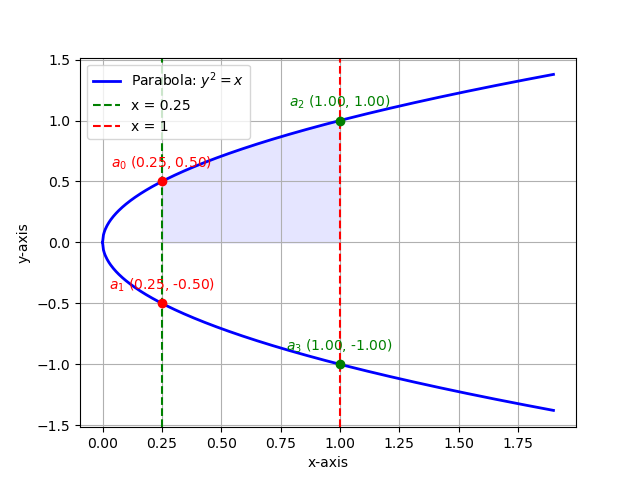
\includegraphics[width=0.7\textwidth]{figs/figasgn3.png}
\end{figure}

\end{document}
